\documentclass[prl,twocolumn,superscriptaddress,showpacs]{revtex4-2}
\usepackage{graphicx}
\usepackage{amsmath,amssymb}
\usepackage{bm}
\usepackage[colorlinks=true,linkcolor=blue,citecolor=blue,urlcolor=blue]{hyperref}
\graphicspath{{figures/}}
\newcommand{\um}{\,\mu\mathrm{m}}
\newcommand{\umi}{\,\mu\mathrm{m}^{-2}}

\begin{document}

\title{Localized in-gap eigenstates of a $10^4$-vertex disordered photonic network from direct interior Maxwell eigensolves}

\author{F. Hern\'andez}
\affiliation{[affiliation to be filled]}

\date{\today}

\begin{abstract}
Bottom-up (611 bands, validated against MPB at $64^3$) and interior (133 certified pairs near eigenvalue index 5000, validated against it) Maxwell eigensolves resolve the gap-edge modes of local-self-uniform photonic networks with $10^3$ and $10^4$ vertices. The $10^3$ gap is empty of eigenvalues; the $10^4$ pseudogap holds ten certified states, five of them bulk-localized with $\xi=1.8$--$2.5\um\ll L=24.6\um$ and persistent under periodic boundary wrapping. Decay lengths funnel to $\sim2\um$ at the edges; level statistics are GOE-like in the bands, Poisson-compatible in 12 levels at the lower edge. No mobility edge is claimed.
\end{abstract}

\maketitle

\emph{Motivation.}---Local-self-uniform (LSU) networks are disordered trivalent dielectric networks that open a full three-dimensional photonic band gap without long-range order~\cite{Sellers2017}, in the family of amorphous-diamond~\cite{Edagawa2008,Imagawa2010} and hyperuniform~\cite{Florescu2009,Man2013,Liew2011,Muller2014,Muller2017,Klatt2019} photonic materials. Gap formation and Anderson localization~\cite{Anderson1958,Abrahams1979} in such correlated disordered media are linked~\cite{John1987,FroufePerez2017}, and a transition from diffusion to localization near the band edge has been observed in 3-D amorphous networks~\cite{Haberko2020}, but the eigenmodes \emph{inside} and at the edges of the gap at the $10^4$-vertex scale have not been resolved by direct computation. Sellers \emph{et al.}\ state that an $N$-vertex supercell has its gap between bands $N/2$ and $N/2+1$~\cite{Sellers2017}, consistent with the band count of the parent gyroid/srs crystal~\cite{Lu2013}, so at $N=10^4$ the gap sits at eigenvalue index $\approx 5000$; computing all lower bands bottom-up would need $1.38$~TB of locked vectors at $256^3$ and $O(100)$ days, hence an interior method.

\emph{System and operator.}---We use the $N=1000$ reference network of Ref.~\cite{Sellers2017} (box $L=11.44\um$, mean rod length $0.80\um$) and an $N=10^4$ network generated with the same protocol at the same vertex density ($0.668\um^{-3}$, $L=10^{1/3}\times11.44=24.647\um$). Rods are rasterized as binary voxels (no subpixel smoothing~\cite{Farjadpour2006,Kottke2008}) in two decorations: the ``elliptical'' convention of the original $N=1000$ montage (radius $0.2252\um$ in a $z$-space stretched by 2.5; $n=2.9275$, $\varepsilon=8.57$; filling fraction $\mathrm{ff}=21.7\%$), and a ``circular'' decoration (radius $0.331836\um$, $n=2.9$, $\varepsilon=8.41$) whose radius was bisected to $\mathrm{ff}=22.00\%$ at $256^3$ (22.01\% at $192^3$; 21.91\% at $128^3$ for $N=1000$). Following MPB~\cite{Johnson2001} we solve $\Theta\bm H=\nabla\times\varepsilon^{-1}\nabla\times\bm H=(\omega/c)^2\bm H$ in the two-component transverse plane-wave basis of the supercell at $k=\Gamma$ (six 3-D FFTs per application; the two $\omega=0$ modes removed exactly; $\Theta$ real symmetric on real fields). Eigenvalues are quoted as $\lambda=(\omega/c)^2$ in $\umi$ and as $\nu=\omega a/2\pi c$ with $a=L/5=2.288\um$ (density-equivalent 8-vertex cell, the same for both sizes). Band numbering is MPB's (bands 1--2 are the $\omega=0$ pair).

\emph{Method.}---(a) For $N=1000$ we use a deflated block LOBPCG~\cite{Knyazev2001,Duersch2018} with MPB's transverse-projection preconditioner~\cite{Johnson2001}, blocks of 32 with 12 guard vectors, complex64 on the GPU with fp64 host Gram/Rayleigh--Ritz algebra (TF32 disabled), per-band relative residual $\le10^{-4}$, and a host-streamed locked set. On identical $64^3$ grids it reproduces MPB (fp64, tolerance $10^{-7}$): max $\Delta\omega/\omega=9.0\times10^{-6}$ over 298 bands and $3.5\times10^{-5}$ over 658 bands (medians $1.4\times10^{-6}$). The pre-registered convergence gate failed as registered: over $64^3/96^3/128^3$ the gap-edge band 500 is non-monotone with a $0.27\%$ spread (three orders of magnitude above the solver--MPB error: rasterization-limited; the other five sampled bands converge monotonically) and the elliptical gap width runs $2.35\to1.93\to2.08\%$. (b) For $N=10^4$ we locate the gap with the kernel polynomial method~\cite{Weisse2006,Lin2016} (KPM; $256^3$, degree 12\,000, 12 probes, Jackson kernel) and solve the window $\lambda\in[1.757,2.117]$ at $192^3$ by two-stage bandpass Chebyshev filtered subspace iteration~\cite{Zhou2006,Pieper2016,Li2019,Winkelmann2019}: a Jackson step-difference filter of degree 3000--4000 builds a basis of $1.5\times$ the predicted count from random starts and the same filter at degree 12\,000 polishes it; candidates are extracted only by fp64 Rayleigh--Ritz on the original $\Theta$ and accepted only if their relative residual on $\Theta$ is $\le10^{-4}$, which by Weyl's inequality places a true eigenvalue within $10^{-4}\lambda$ of every accepted value (spurious eigenvalues are thereby excluded; eigenvectors of the two pairs closer than that are certified only as a two-dimensional span). It won a measured bake-off on a 50-band interior slice of the exact $N=1000$ spectrum (24/50 verified within budget vs 0/50) against folded-spectrum LOBPCG~\cite{Wang1994,Vomel2008} and shift-invert PMINRES at the tested budgets; filtered Lanczos~\cite{FangSaad2012} was excluded on memory grounds [Supplemental Material (SM)~\cite{SM}]. Its accuracy is set by re-solving that slice in the production configuration (polish degree 8000 rather than 12\,000): $50/50$ found, 0 ghosts, max $\Delta\lambda/\lambda=2.4\times10^{-7}$ (median $6\times10^{-8}$)---after correcting a Rayleigh-quotient normalization bug that biased every eigenvalue high by $+4.7\times10^{-5}$ ($\lambda_{\rm corr}=\lambda_{\rm raw}/\|x\|^2$, applied retroactively; SM)---and by an independent cross-check on the circular $N=1000$ decoration ($210/210$ states, max $4.1\times10^{-7}$). Localization is quantified per mode from $u=\varepsilon|\bm E|^2$ by the participation fraction $p=(\sum u)^2/(N_{\rm vox}\sum u^2)$ and an envelope decay length $\xi$ from a linear fit of $\ln u(r)$ vs the (minimum-image) distance $r$ from the peak over $[0.10,0.95]\,L/2$, $u\propto e^{-2r/\xi}$; a fit is ``unresolved'' (lower bound only) if $\xi\ge L/2$, if $u$ decays by less than one decade, or if $r^2<0.7$.

\begin{figure*}
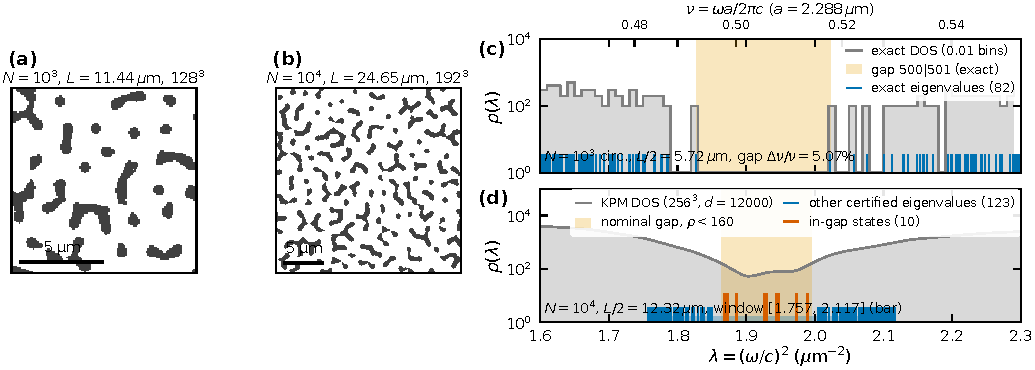
\includegraphics[width=\textwidth]{fig1_structure_dos}
\caption{(a,b) Mid-plane $\varepsilon(\bm r)$ of the $N=10^3$ ($128^3$) and $N=10^4$ ($192^3$) networks, circular decoration (dark = dielectric). (c) $N=10^3$, circular decoration: exact eigenvalues (bottom-up, 611 bands) around the gap and their binned density of states; the shaded band is the exact gap between MPB bands 500 and 501. (d) $N=10^4$: KPM density of states ($256^3$) with the 133 residual-certified $192^3$ eigenvalues (blue) and the ten inside the nominal gap $\rho<160$ states per unit $\lambda$ (red); bar: solved window. Top axis: $\nu=\omega a/2\pi c$, $a=2.288\um$.}
\label{fig1}
\end{figure*}

\emph{Results, $N=1000$.}---All 611 bands (MPB bands 3--613) of the elliptical structure at $128^3$ were solved in 5.5~h; the gap lies between bands 500 and 501 as pre-registered: $\lambda=1.8830\to1.9628\umi$, $\Delta\nu/\nu=2.08\%$ at $128^3$ (centre $\nu=0.505$), a spacing $10\times$ the median of its 20 neighbours. With the circular decoration the gap is again at 500|501 and widens to $1.8276\to2.0225\umi$, $\Delta\nu/\nu=5.07\%$ ($26\times$ the neighbouring spacings). Both gaps are empty of eigenvalues. The regenerated montage matches the original in character (SM). Band-edge modes are localized, deep-window modes extended [Fig.~\ref{fig2}(a)]: circular decoration $\xi=1.47\um$ (band 500, $r^2=0.97$, $p=0.42\%$) and $2.30\um$ (band 501, $p=3.9\%$) vs $p=9$--$37\%$ far from the gap; elliptical $\xi=1.82$ and $2.92\um$. Only 42 of 210 circular-decoration modes have resolved $\xi$ (142 hit the $L/2=5.72\um$ ceiling), the quantitative reason for the $N=10^4$ computation.

\begin{figure*}
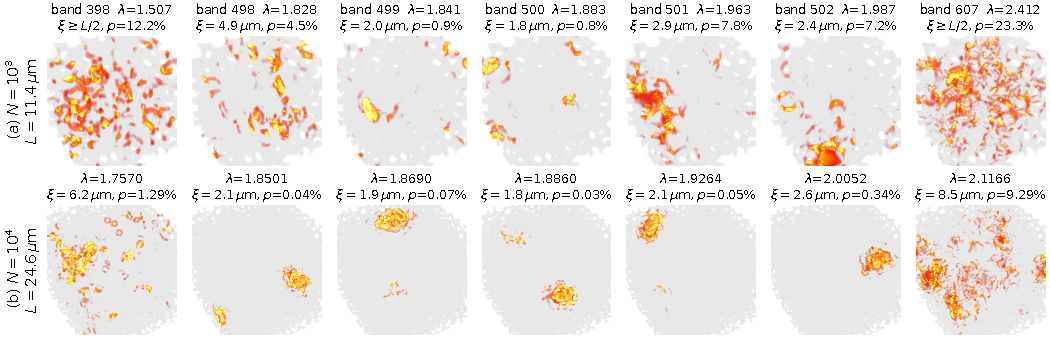
\includegraphics[width=\textwidth]{fig2_tiles}
\caption{Energy density $\varepsilon|\bm E|^2$ (volume render, per-tile colour scale clipped at the 99.9th percentile; network in translucent grey). (a) $N=10^3$, elliptical decoration, bands 398, 498--502, 607 around the 500|501 gap. (b) $N=10^4$, circular decoration: window bottom (1.7570), the nearest state below the nominal gap (1.8501), three of the five in-gap candidates (1.9738 and 1.9901 not shown), the nearest state above it (2.0052), window top (2.1166). $\xi$ and $p$ as defined in the text; ``$\xi\ge L/2$'' marks a ceiling-limited fit.}
\label{fig2}
\end{figure*}

\emph{Results, $N=10^4$.}---KPM places $5010.3\pm12.5$ transverse states below $\lambda=1.957$, i.e.\ $0.501$ bands per vertex, consistent with the $N/2$ rule to $\pm0.3\%$ (gap at MPB bands $\approx5012|5013\pm13$). The Jackson-smoothed KPM density falls below 160 states per unit $\lambda$ over $[1.864,1.996]\umi$ ($\Delta\nu/\nu=3.4\%$; 5\%/20\% criteria: $[1.885,1.968]$/$[1.837,2.022]$, a $\pm0.03$ systematic; certified states inside: 5, 10, 21), narrower than the $5.07\%$ gap of the $N=1000$ box with the same decoration and contained within it. Three overlapping slices at $192^3$ ($69+5+61$ pairs, two duplicates removed by eigenvector overlap) give \textbf{133 residual-certified eigenpairs} in $[1.75705,2.11657]\umi$ (worst residual $5.9\times10^{-5}$; 104 GPU-hours, $1.16\times10^{7}$ operator applications), with no in-window pair left unconverged. Completeness is certified on the sub-interval $[1.9063,1.9606]$ by a deflated-probe KPM count of missed states, $|{\rm missed}|<0.01$ (stochastic s.e.\ $10^{-4}$; the estimator's own floor from modelled leakage and eigenvector error is $\sim3\times10^{-3}$, against a signal of $\approx1$ per missed state); on the full window the same estimator ($+1.7\pm0.3$) carries an edge-leakage bias $\ge1.2\pm0.2$ and is consistent with zero or one missing state (SM). The largest interior spacing of the certified spectrum runs from $1.8860$ to $1.9264\umi$ ($\Delta\nu/\nu=1.06\%$, $28\times$ the median spacing; completeness is certified only above 1.9063); but the nominal gap is not empty. \textbf{Ten certified states lie inside $[1.864,1.996]$}, at $\lambda=1.8690$, 1.8708, 1.8731, 1.8860, 1.9264, 1.9296, 1.9441, 1.9472, 1.9738, 1.9901 [Fig.~\ref{fig1}(d), Table~SI]. Four of them are flagged as boundary-seam states of the rasterization convention: rods whose radius pokes through a box face are not wrapped, so the outermost voxel shell has $\mathrm{ff}=0.1975$ against $0.2211$ inside (an 11\% deficit, a planar defect), and the states at 1.8708, 1.8731, 1.9296, 1.9472 carry 18, 24, 44 and 42\% of their energy in that shell (6.1\% of the volume; three peak on a box edge). Re-solving the gap window with minimum-image wrapping (0.078\% of voxels change) finds no partner for three of them (best overlaps 0.006, 0.131, 0.090), but the periodic solve is itself measured incomplete ($+2.0\pm0.4$ missed), so their absence is likely, not proven; the fourth (1.9472, overlap 0.30) is undetermined. A fifth in-gap state (1.9441) is compact ($p=0.56\%$) but has a non-exponential envelope ($r^2=0.33$, $\xi$ unresolved); its periodic partner (overlap 0.95) fits as $\xi=2.2\um$, and it is excluded from the candidate list conservatively. \textbf{Five bulk-localized in-gap states remain} among the certified set: $\xi=1.80$--$2.51\um$ ($\xi/L=0.07$--$0.10$), $p=0.034$--$0.33\%$ (participation volumes 5--49$\um^3$ in a $15\,000\um^3$ box), $r^2=0.971$--$0.998$, shell energy 2.5--10.5\%; all five persist under periodic wrapping with overlaps 0.968--1.000 and shifts $\Delta\lambda=-0.0007$ to $-0.0030$, every shift negative as required when dielectric is added. A $2.4\times$ voxel refinement ($256^3$) on two anchor windows matched 11 of 11 states in $[1.84,1.95]$ one-to-one by eigenvector overlap (min 0.873, median 0.996, the two lowest a rotating near-degenerate pair; $|\Delta\omega/\omega|\le0.34\%$) and 10 of 11 in $[1.99,2.035]$ ($\le0.04\%$, an upper bound: 3 of 11 fine pairs certified, the rest carrying a Weyl uncertainty $\le0.011\%$). Three candidates (1.8690, 1.8860, 1.9264) lie in the low anchor and persist; 1.9738 was not tested, and 1.9901, at the high-anchor floor, has no fine partner. This is good evidence against a rasterization artefact for the tested states; with 7.8 voxels/$\mu$m and the 0.27\% spread seen at $N=1000$, sub-percent gap-edge frequencies are not claimed.

The decay length varies smoothly across the window [Fig.~\ref{fig3}(a)]: 121 of 133 fits are resolved (12 fail $r^2\ge0.7$), and the medians by spectral bin are $5.0\to3.0\to2.1\um$ approaching the lower edge, $2.1\um$ inside, and $2.8\to4.7\to6.1\um$ climbing away above; $p$ spans $0.03$--$12\%$ [Fig.~\ref{fig3}(b)], and the participation-volume radius $(3V_p/4\pi)^{1/3}$ follows the same funnel ($2.7\to1.5\to1.2\um$ and $1.4\to3.1\to4.1\to5.4\um$). The envelope fit is not a precision quantity: shrinking the fit range to $[0.10,0.60]\,L/2$ moves $\xi$ by a median 30\% and the window-end/near-edge contrast from $1.7$--$2.2\times$ to $1.6$--$1.8\times$; the funnel is robust, three-figure $\xi$ values are not.

\begin{figure}
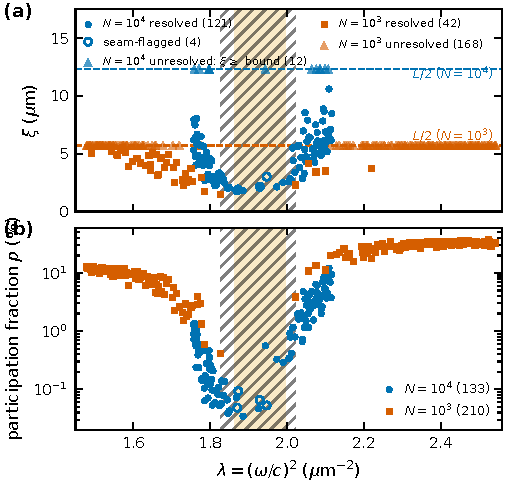
\includegraphics[width=\columnwidth]{fig3_xi_pr}
\caption{(a) Envelope decay length $\xi$ vs $\lambda$ for $N=10^4$ (circles, $192^3$) and $N=10^3$ circular decoration (squares, $128^3$); dashed lines are the finite-size ceilings $L/2$; triangles at the ceiling are unresolved fits (lower bounds); open circles are the four seam-flagged states; shaded: nominal $N=10^4$ gap; hatched: $N=10^3$ gap. (b) Participation fraction. Same decoration for both sizes.}
\label{fig3}
\end{figure}

\emph{Can we claim Anderson localization?}---We take the items in turn. (1)~\emph{Spatial localization}: supported. The five bulk in-gap candidates have $\xi=1.8$--$2.5\um$ in $L=24.6\um$, $p\le0.33\%$ and $r^2\ge0.97$; the tiles [Fig.~\ref{fig2}(b)] are single compact blobs a few $\mu$m across. $\xi$ is an envelope-fit length with tens-of-percent fit-range sensitivity, not a transport length. (2)~\emph{Interference-driven (Anderson) vs trap-like (Lifshitz-tail~\cite{Lifshitz1964}) states}: not separable with this data. Both boxes are single realizations with the same local statistics (ff coarse-grained at $2\um$: 0.2204 vs 0.2209, s.d.\ 0.0398 vs 0.0405) but $N=10^4$ has ten times as many $\xi$-cells; at 5 in-gap states per $N=10^4$ volume an empty $N=1000$ gap has probability $e^{-0.5}=0.61$---but over the interval $[1.8276,2.0225]$ where the $N=1000$ gap is actually empty the $N=10^4$ spectrum holds 19 bulk states, giving $e^{-1.9}\approx0.15$, so the statistics argument is plausible, not compelling. A direct test (energy-weighted local filling fraction of candidates vs bulk controls) was run and \emph{retracted}: unmatched in mode extent, it reverses against an extent-matched null (SM). Neither origin is established. (3)~\emph{Finite-size scaling}: two sizes only. Matched-decoration band-edge states have $\xi=1.47$ and $2.30\um$ at $L=11.44\um$ and $1.80$ and $2.09\um$ at $L=24.65\um$ [edge states 1.8860 and 1.9264; Fig.~\ref{fig4}(b)], with participation volumes $6$ and $58\um^3$ vs $5$ and $7\um^3$: $\xi$ is $L$-independent within the fit uncertainty, but at the estimator's 30\% systematic this two-point test has little discriminating power (the upper-edge participation volumes differ by $8\times$), two points are not a scaling analysis, and 168 of 210 $N=1000$ fits are unresolved (142 at the ceiling). (4)~\emph{Level statistics}~\cite{Shklovskii1993,Evers2008}: $\Theta$ at $\Gamma$ with real $\varepsilon$ is real symmetric, so the class is orthogonal: $\langle r\rangle_{\rm P}=2\ln2-1=0.386$, $\langle r\rangle_{\rm GOE}=0.531$~\cite{Oganesyan2007,Atas2013}. The adjacent-gap ratio (no unfolding needed) is computed within contiguous bands [Fig.~\ref{fig4}(a)]. In the extended regions it is GOE-like: $0.528\pm0.038$ (51 levels, $\lambda<1.816$) and $0.528\pm0.041$ (42 levels, $\lambda>2.05$) at $N=10^4$, pooled $0.519\pm0.024$ outside the bracket; $0.508\pm0.010$ and $0.533\pm0.011$ over all 611 $N=1000$ levels (elliptical, circular). In the 12 levels just below the gap ($1.8208\le\lambda\le1.8502$, a post-hoc window), where $\xi=2.0$--$3.4\um$, $\langle r\rangle=0.357\pm0.073$, $2.2\sigma$ below the GOE expectation for 12 levels and consistent with Poisson; four of these 12 levels carry outer-shell enhancement $>2\times$ (up to 25\%, comparable to the seam-flagged in-gap states) and are not excluded. Above the gap the 18 nearest levels ($2.005$--$2.050$, $p\approx1\%$, $\xi$ median $3.5\um$) give $0.559\pm0.047$: comparably compact states show repulsion there, an unexplained asymmetry. The ten in-gap levels give $0.31\pm0.08$, but ten levels, four of them seam-flagged, are not a statistic. Uncertainties are bootstrap. The residual gate guarantees $|\Delta\lambda|\le10^{-4}\lambda\approx1.9\times10^{-4}\umi$ per level (Weyl), 14\% of the median spacing $1.4\times10^{-3}\umi$, while the accuracy measured on the $N=1000$ ground truth is $\Delta\lambda/\lambda\le4\times10^{-7}$ and duplicate states found by two slices agree to $10^{-8}$; a single missing level would move the 12-level ratio by $\lesssim0.03$. Level repulsion where states are extended and its loss where they are localized is the expected pattern, but the near-edge samples are small, post hoc and seam-contaminated: suggestive, not conclusive. A Thouless-type sensitivity to boundary twists cannot be obtained from the saved $\Gamma$-point data. (5)~\emph{Mobility edge}: not claimable---no transport, one realization per size, no scaling; the $\xi(\omega)$ funnel (Fig.~\ref{fig3}) and the $\langle r\rangle$ drop [Fig.~\ref{fig4}(a)] are the \emph{phenomenology} of a localization--delocalization crossover at the gap edge, the regime probed experimentally in 3-D amorphous networks~\cite{Haberko2020} and predicted for correlated disorder~\cite{FroufePerez2017}. (6)~\emph{Vector-wave caveat}: early reports of 3-D localization of light~\cite{Wiersma1997} were not confirmed, vector waves do not localize in uncorrelated point-scatterer ensembles~\cite{Skipetrov2014,Sperling2016,SkipetrovPage2016}, and numerical 3-D localization has been shown only for overlapping metallic, not dielectric, spheres~\cite{Yamilov2023}; localization at the edge of a photonic gap in a correlated network~\cite{John1984,John1987,FroufePerez2017} is a different mechanism; this data addresses only the spatial structure of the eigenstates at such an edge.

\begin{figure}
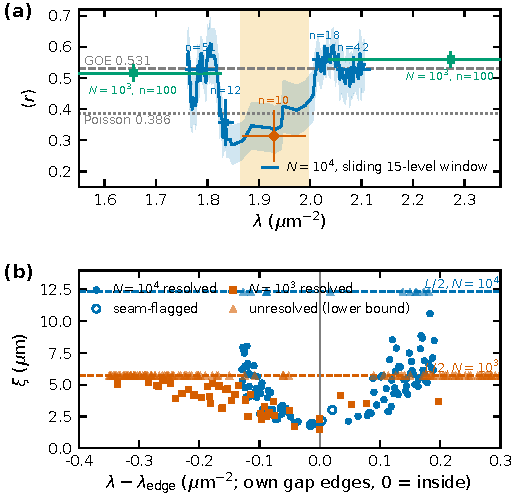
\includegraphics[width=\columnwidth]{fig4_localization_stats}
\caption{(a) Adjacent-gap ratio $\langle r\rangle$: $N=10^4$ sliding 15-level window (line, $\pm1$ s.e.; inside the bracket it includes the seam-flagged levels and ratios dominated by the two largest spacings, and is not interpreted) and contiguous bands (circles: 51, 12, 18, 42 levels; diamond: ten in-gap levels; bootstrap errors); $N=10^3$ circular, bands 401--500 and 501--600 (squares). Dashed/dotted: GOE 0.531 / Poisson 0.386. (b) Matched-decoration comparison: resolved $\xi$ vs distance from each box's own gap edges ($N=10^3$: 1.8276|2.0225; $N=10^4$: 1.8860|1.9264; in-gap states at 0).}
\label{fig4}
\end{figure}

\emph{Verdict.}---The defensible claim is: strongly spatially localized in-gap and gap-edge eigenstates with $\xi\ll L$, with the two resolved $N=1000$ band-edge values in the same range, consistent with localization at the edges of a photonic pseudogap in a correlated disordered network, accompanied by GOE-like level statistics in the extended bands and a Poisson-compatible ratio in 12 post-hoc levels at the lower edge that is not reproduced above the gap. Whether these states are interference-driven (Anderson-type) or trapped in rare local configurations (Lifshitz-tail-type) cannot be decided from this data. The claim of an Anderson transition or a mobility edge requires finite-size scaling over three or more sizes and/or transport or larger-sample level statistics that this data does not contain.

\emph{Limitations.}---Gap-edge frequencies are rasterization-limited (0.27\% non-monotone spread at $N=1000$; $\le0.34\%$ between $192^3$ and $256^3$ at $N=10^4$), and on MPB's interpolated read-back of the $64^3$ grid the elliptical 500|501 spacing is 0.60\% (largest at 501|502), so the gap position at $64^3$ is convention-dependent. Decay lengths are bounded by $L/2$ and fit-range dependent at the 30\% level; one disorder realization per size. Arithmetic is fp32 on the device with fp64 Rayleigh--Ritz; the merged 133-mode set is orthonormal only to $4.9\times10^{-4}$ across independently solved slices ($8.6\times10^{-6}$ within), the level the $10^{-4}$ residual gate permits, which affects no spectrum, montage or localization result. Twenty of the 133 modes have outer-shell enhancement $>2\times$; only the four inside the bracket were re-solved seam-free. Of the statements withdrawn during the project (eight are listed in the SM), four bear on the results here and are absent: the rare-region $z$-test, the statement that the resolution confound is ``closed'' (its power-retention statistic is saturated), the ``vanished'' verdict for the state at 1.9472, and all uncorrected eigenvalues. Full records and every number with its source file are in the SM~\cite{SM}.

\begin{acknowledgments}
[Acknowledgments to be filled.]
\end{acknowledgments}

\bibliographystyle{apsrev4-2}
\bibliography{refs}

\end{document}
